% Figure: KG agent (production) vs in-context surface forms.
% Mean of typedb+neo4j vs mean of C-TQL/Cypher/NL/JSONLD per LLM.
\begin{figure}[t]
\centering
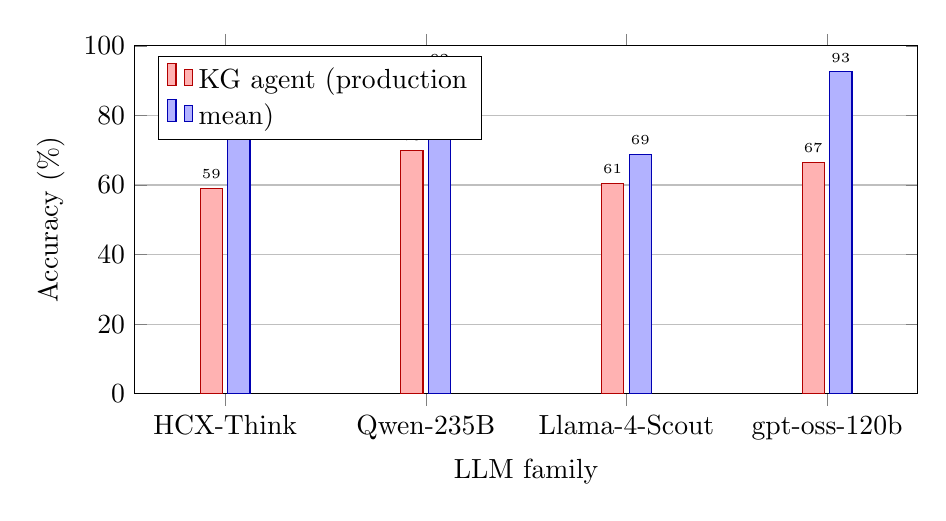
\begin{tikzpicture}
\begin{axis}[
  width=0.95\textwidth,
  height=6cm,
  ybar=2pt,
  bar width=8pt,
  ymin=0, ymax=100,
  ymajorgrids=true,
  ylabel={Accuracy (\%)},
  xlabel={LLM family},
  symbolic x coords={HCX-Think, Qwen-235B, Llama-4-Scout, gpt-oss-120b},
  xtick=data,
  legend pos=north west,
  legend cell align=left,
  enlarge x limits=0.15,
  nodes near coords,
  nodes near coords align={vertical},
  nodes near coords style={font=\tiny},
  every node near coord/.append style={/pgf/number format/.cd, fixed, precision=0},
]
% KG-agent mean = (typedb + neo4j) / 2
\addplot[fill=red!30, draw=red!70!black] coordinates {
  (HCX-Think, 59) (Qwen-235B, 70) (Llama-4-Scout, 60.5) (gpt-oss-120b, 66.5)
};
% In-context mean = (TQL + Cypher + NL + JSONLD) / 4
\addplot[fill=blue!30, draw=blue!70!black] coordinates {
  (HCX-Think, 87.75) (Qwen-235B, 92) (Llama-4-Scout, 68.75) (gpt-oss-120b, 92.5)
};
\legend{KG agent (production, mean), In-context surface form (mean)}
\end{axis}
\end{tikzpicture}
\caption{Production KG-RAG agents (mean of \backendname{typedb} and
\backendname{neo4j}) vs.\ in-context surface-form ablation
(mean of \backendname{C-TQL}, \backendname{C-Cypher}, \backendname{C-NL},
\backendname{C-JSONLD}). The in-context surface forms outperform the
production KG agents in all four LLM families, despite the KG agents
having access to a strictly larger graph (more entities and relations
than the dump). The gap ranges from 8 percentage points
(Llama-4-Scout, where the in-context tier is itself dragged down by KG
syntax familiarity) to 26 percentage points (gpt-oss-120b).}
\label{fig:kg-vs-incontext}
\end{figure}
